% Options for packages loaded elsewhere
\PassOptionsToPackage{unicode}{hyperref}
\PassOptionsToPackage{hyphens}{url}
\PassOptionsToPackage{dvipsnames,svgnames,x11names}{xcolor}
%
\documentclass[
  letterpaper,
  DIV=11,
  numbers=noendperiod]{scrreprt}

\usepackage{amsmath,amssymb}
\usepackage{iftex}
\ifPDFTeX
  \usepackage[T1]{fontenc}
  \usepackage[utf8]{inputenc}
  \usepackage{textcomp} % provide euro and other symbols
\else % if luatex or xetex
  \usepackage{unicode-math}
  \defaultfontfeatures{Scale=MatchLowercase}
  \defaultfontfeatures[\rmfamily]{Ligatures=TeX,Scale=1}
\fi
\usepackage{lmodern}
\ifPDFTeX\else  
    % xetex/luatex font selection
\fi
% Use upquote if available, for straight quotes in verbatim environments
\IfFileExists{upquote.sty}{\usepackage{upquote}}{}
\IfFileExists{microtype.sty}{% use microtype if available
  \usepackage[]{microtype}
  \UseMicrotypeSet[protrusion]{basicmath} % disable protrusion for tt fonts
}{}
\makeatletter
\@ifundefined{KOMAClassName}{% if non-KOMA class
  \IfFileExists{parskip.sty}{%
    \usepackage{parskip}
  }{% else
    \setlength{\parindent}{0pt}
    \setlength{\parskip}{6pt plus 2pt minus 1pt}}
}{% if KOMA class
  \KOMAoptions{parskip=half}}
\makeatother
\usepackage{xcolor}
\setlength{\emergencystretch}{3em} % prevent overfull lines
\setcounter{secnumdepth}{-\maxdimen} % remove section numbering
% Make \paragraph and \subparagraph free-standing
\ifx\paragraph\undefined\else
  \let\oldparagraph\paragraph
  \renewcommand{\paragraph}[1]{\oldparagraph{#1}\mbox{}}
\fi
\ifx\subparagraph\undefined\else
  \let\oldsubparagraph\subparagraph
  \renewcommand{\subparagraph}[1]{\oldsubparagraph{#1}\mbox{}}
\fi

\usepackage{color}
\usepackage{fancyvrb}
\newcommand{\VerbBar}{|}
\newcommand{\VERB}{\Verb[commandchars=\\\{\}]}
\DefineVerbatimEnvironment{Highlighting}{Verbatim}{commandchars=\\\{\}}
% Add ',fontsize=\small' for more characters per line
\usepackage{framed}
\definecolor{shadecolor}{RGB}{241,243,245}
\newenvironment{Shaded}{\begin{snugshade}}{\end{snugshade}}
\newcommand{\AlertTok}[1]{\textcolor[rgb]{0.68,0.00,0.00}{#1}}
\newcommand{\AnnotationTok}[1]{\textcolor[rgb]{0.37,0.37,0.37}{#1}}
\newcommand{\AttributeTok}[1]{\textcolor[rgb]{0.40,0.45,0.13}{#1}}
\newcommand{\BaseNTok}[1]{\textcolor[rgb]{0.68,0.00,0.00}{#1}}
\newcommand{\BuiltInTok}[1]{\textcolor[rgb]{0.00,0.23,0.31}{#1}}
\newcommand{\CharTok}[1]{\textcolor[rgb]{0.13,0.47,0.30}{#1}}
\newcommand{\CommentTok}[1]{\textcolor[rgb]{0.37,0.37,0.37}{#1}}
\newcommand{\CommentVarTok}[1]{\textcolor[rgb]{0.37,0.37,0.37}{\textit{#1}}}
\newcommand{\ConstantTok}[1]{\textcolor[rgb]{0.56,0.35,0.01}{#1}}
\newcommand{\ControlFlowTok}[1]{\textcolor[rgb]{0.00,0.23,0.31}{#1}}
\newcommand{\DataTypeTok}[1]{\textcolor[rgb]{0.68,0.00,0.00}{#1}}
\newcommand{\DecValTok}[1]{\textcolor[rgb]{0.68,0.00,0.00}{#1}}
\newcommand{\DocumentationTok}[1]{\textcolor[rgb]{0.37,0.37,0.37}{\textit{#1}}}
\newcommand{\ErrorTok}[1]{\textcolor[rgb]{0.68,0.00,0.00}{#1}}
\newcommand{\ExtensionTok}[1]{\textcolor[rgb]{0.00,0.23,0.31}{#1}}
\newcommand{\FloatTok}[1]{\textcolor[rgb]{0.68,0.00,0.00}{#1}}
\newcommand{\FunctionTok}[1]{\textcolor[rgb]{0.28,0.35,0.67}{#1}}
\newcommand{\ImportTok}[1]{\textcolor[rgb]{0.00,0.46,0.62}{#1}}
\newcommand{\InformationTok}[1]{\textcolor[rgb]{0.37,0.37,0.37}{#1}}
\newcommand{\KeywordTok}[1]{\textcolor[rgb]{0.00,0.23,0.31}{#1}}
\newcommand{\NormalTok}[1]{\textcolor[rgb]{0.00,0.23,0.31}{#1}}
\newcommand{\OperatorTok}[1]{\textcolor[rgb]{0.37,0.37,0.37}{#1}}
\newcommand{\OtherTok}[1]{\textcolor[rgb]{0.00,0.23,0.31}{#1}}
\newcommand{\PreprocessorTok}[1]{\textcolor[rgb]{0.68,0.00,0.00}{#1}}
\newcommand{\RegionMarkerTok}[1]{\textcolor[rgb]{0.00,0.23,0.31}{#1}}
\newcommand{\SpecialCharTok}[1]{\textcolor[rgb]{0.37,0.37,0.37}{#1}}
\newcommand{\SpecialStringTok}[1]{\textcolor[rgb]{0.13,0.47,0.30}{#1}}
\newcommand{\StringTok}[1]{\textcolor[rgb]{0.13,0.47,0.30}{#1}}
\newcommand{\VariableTok}[1]{\textcolor[rgb]{0.07,0.07,0.07}{#1}}
\newcommand{\VerbatimStringTok}[1]{\textcolor[rgb]{0.13,0.47,0.30}{#1}}
\newcommand{\WarningTok}[1]{\textcolor[rgb]{0.37,0.37,0.37}{\textit{#1}}}

\providecommand{\tightlist}{%
  \setlength{\itemsep}{0pt}\setlength{\parskip}{0pt}}\usepackage{longtable,booktabs,array}
\usepackage{calc} % for calculating minipage widths
% Correct order of tables after \paragraph or \subparagraph
\usepackage{etoolbox}
\makeatletter
\patchcmd\longtable{\par}{\if@noskipsec\mbox{}\fi\par}{}{}
\makeatother
% Allow footnotes in longtable head/foot
\IfFileExists{footnotehyper.sty}{\usepackage{footnotehyper}}{\usepackage{footnote}}
\makesavenoteenv{longtable}
\usepackage{graphicx}
\makeatletter
\def\maxwidth{\ifdim\Gin@nat@width>\linewidth\linewidth\else\Gin@nat@width\fi}
\def\maxheight{\ifdim\Gin@nat@height>\textheight\textheight\else\Gin@nat@height\fi}
\makeatother
% Scale images if necessary, so that they will not overflow the page
% margins by default, and it is still possible to overwrite the defaults
% using explicit options in \includegraphics[width, height, ...]{}
\setkeys{Gin}{width=\maxwidth,height=\maxheight,keepaspectratio}
% Set default figure placement to htbp
\makeatletter
\def\fps@figure{htbp}
\makeatother

\KOMAoption{captions}{tableheading}
\makeatletter
\@ifpackageloaded{tcolorbox}{}{\usepackage[skins,breakable]{tcolorbox}}
\@ifpackageloaded{fontawesome5}{}{\usepackage{fontawesome5}}
\definecolor{quarto-callout-color}{HTML}{909090}
\definecolor{quarto-callout-note-color}{HTML}{0758E5}
\definecolor{quarto-callout-important-color}{HTML}{CC1914}
\definecolor{quarto-callout-warning-color}{HTML}{EB9113}
\definecolor{quarto-callout-tip-color}{HTML}{00A047}
\definecolor{quarto-callout-caution-color}{HTML}{FC5300}
\definecolor{quarto-callout-color-frame}{HTML}{acacac}
\definecolor{quarto-callout-note-color-frame}{HTML}{4582ec}
\definecolor{quarto-callout-important-color-frame}{HTML}{d9534f}
\definecolor{quarto-callout-warning-color-frame}{HTML}{f0ad4e}
\definecolor{quarto-callout-tip-color-frame}{HTML}{02b875}
\definecolor{quarto-callout-caution-color-frame}{HTML}{fd7e14}
\makeatother
\makeatletter
\makeatother
\makeatletter
\makeatother
\makeatletter
\@ifpackageloaded{caption}{}{\usepackage{caption}}
\AtBeginDocument{%
\ifdefined\contentsname
  \renewcommand*\contentsname{Table of contents}
\else
  \newcommand\contentsname{Table of contents}
\fi
\ifdefined\listfigurename
  \renewcommand*\listfigurename{List of Figures}
\else
  \newcommand\listfigurename{List of Figures}
\fi
\ifdefined\listtablename
  \renewcommand*\listtablename{List of Tables}
\else
  \newcommand\listtablename{List of Tables}
\fi
\ifdefined\figurename
  \renewcommand*\figurename{Figure}
\else
  \newcommand\figurename{Figure}
\fi
\ifdefined\tablename
  \renewcommand*\tablename{Table}
\else
  \newcommand\tablename{Table}
\fi
}
\@ifpackageloaded{float}{}{\usepackage{float}}
\floatstyle{ruled}
\@ifundefined{c@chapter}{\newfloat{codelisting}{h}{lop}}{\newfloat{codelisting}{h}{lop}[chapter]}
\floatname{codelisting}{Listing}
\newcommand*\listoflistings{\listof{codelisting}{List of Listings}}
\makeatother
\makeatletter
\@ifpackageloaded{caption}{}{\usepackage{caption}}
\@ifpackageloaded{subcaption}{}{\usepackage{subcaption}}
\makeatother
\makeatletter
\@ifpackageloaded{tcolorbox}{}{\usepackage[skins,breakable]{tcolorbox}}
\makeatother
\makeatletter
\@ifundefined{shadecolor}{\definecolor{shadecolor}{rgb}{.97, .97, .97}}
\makeatother
\makeatletter
\makeatother
\makeatletter
\makeatother
\ifLuaTeX
  \usepackage{selnolig}  % disable illegal ligatures
\fi
\IfFileExists{bookmark.sty}{\usepackage{bookmark}}{\usepackage{hyperref}}
\IfFileExists{xurl.sty}{\usepackage{xurl}}{} % add URL line breaks if available
\urlstyle{same} % disable monospaced font for URLs
\hypersetup{
  colorlinks=true,
  linkcolor={blue},
  filecolor={Maroon},
  citecolor={Blue},
  urlcolor={Blue},
  pdfcreator={LaTeX via pandoc}}

\author{}
\date{}

\begin{document}
\ifdefined\Shaded\renewenvironment{Shaded}{\begin{tcolorbox}[frame hidden, interior hidden, enhanced, sharp corners, borderline west={3pt}{0pt}{shadecolor}, boxrule=0pt, breakable]}{\end{tcolorbox}}\fi

\hypertarget{ux6bcdux96c6ux56e3ux3068ux6a19ux672c}{%
\section{母集団と標本}\label{ux6bcdux96c6ux56e3ux3068ux6a19ux672c}}

\hypertarget{ux306fux3058ux3081ux306b}{%
\section{はじめに}\label{ux306fux3058ux3081ux306b}}

\begin{itemize}
\item
  社会調査や学術研究では,知りたい対象と手元のデータが必ずしも一致していません。そもそも,知りたい対象全体のデータを取るような調査はほとんど行われません。

  \begin{itemize}
  \tightlist
  \item
    唯一の例外は国勢調査
  \end{itemize}
\item
  例えば,世論調査は日本在住者の政治に対する意見などを知るためにデータを集めますが,全国民を対象としているわけではありません。

  \begin{itemize}
  \item
    全国民の意見を聞いていたら時間もお金もかかります。そもそも全員と連絡をつけることは非現実的です。
  \item
    そこで,例えば1,000人に聞いた意見から日本全体の世論を推測します。
  \end{itemize}
\item
  例えば,新しい薬の効果を検証したい場合,知りたい対象は,過去・現在・未来に渡る特定の病気の患者への効果です。調査時点で過去の患者や未来の患者に対する効果を知ることはできません。

  \begin{itemize}
  \tightlist
  \item
    そこで,治験対象者のデータから,人類一般に対する効果を推測します。
  \end{itemize}
\item
  ここで,知りたい対象を\textbf{母集団},検証に使う母集団の一部を\textbf{標本}と言います。
\end{itemize}

\begin{tcolorbox}[enhanced jigsaw, title=\textcolor{quarto-callout-note-color}{\faInfo}\hspace{0.5em}{Note}, colframe=quarto-callout-note-color-frame, bottomrule=.15mm, colback=white, left=2mm, leftrule=.75mm, opacitybacktitle=0.6, breakable, arc=.35mm, rightrule=.15mm, titlerule=0mm, colbacktitle=quarto-callout-note-color!10!white, bottomtitle=1mm, opacityback=0, coltitle=black, toptitle=1mm, toprule=.15mm]

特に経済学などでは,上記1つ目の例のように日本人全体,といった特定の母集団を想定しないことが多いとされます(星野ほか
2023; 高橋
2022)。その代わりに,サンプルを生み出す特定の確率分布を母集団と呼びます。

\end{tcolorbox}

\begin{itemize}
\item
  確率論を基礎として,十分な数の適切に選ばれた標本を適切な方法で分析すると,非常に高い精度で母集団の傾向を推測できることが知られています。
\item
  ただし,「適切に標本を選ぶこと」「適切に分析すること」は現実にそう簡単ではなく,それゆえこの授業で扱う多変量解析を含め,多くの統計理論が研究され続けています。
\end{itemize}

まずは,理想的な状況における推測について扱います。

\hypertarget{ux5e73ux5747ux3068ux5206ux6563ux5fa9ux7fd2ux3b1}{%
\section{平均と分散(復習+α)}\label{ux5e73ux5747ux3068ux5206ux6563ux5fa9ux7fd2ux3b1}}

\begin{itemize}
\tightlist
\item
  平均はデータの特徴を表す代表的な値の一つでした。変数 \(X\) の平均
  \(\bar X\)は,
\end{itemize}

\[ \bar X = (X_1 + X_2 + ... X_n )/n = \frac{1}{n} \Sigma_{i=1}^{n} X_i
\]

\begin{itemize}
\tightlist
\item
  分散はデータのばらつきを表します。データは平均より高かったり低かったりするので,各データの平均からのずれ
  \((X_i - \bar X)\)を2乗して
\end{itemize}

\[
\begin{split}
s_X^2 &= \frac{1}{n-1}\{(X_1 - \bar X)^2+(X_2 - \bar X)^2+(X_3 - \bar X)^2+...(X_n - \bar X)^2 \} \\ &= \frac{1}{n-1}\Sigma (X_i - \bar X)^2
\end{split}
\]

\begin{tcolorbox}[enhanced jigsaw, breakable, arc=.35mm, colframe=quarto-callout-caution-color-frame, bottomrule=.15mm, colback=white, left=2mm, leftrule=.75mm, opacityback=0, rightrule=.15mm, toprule=.15mm]

前回と違って,\(n-1\)で割っています。前回のものを標本分散,今回のものを不偏分散と言います。標本を使って母集団の分散を推定する際には,不偏分散の方が良い(より正確になる)ためです。

\end{tcolorbox}

\hypertarget{ux6a19ux672cux5e73ux5747ux306eux6027ux8cea}{%
\section{標本平均の性質}\label{ux6a19ux672cux5e73ux5747ux306eux6027ux8cea}}

\begin{itemize}
\item
  ある母集団から得た標本があります。母集団全体の平均(母平均)を \(\mu\)
  とします。この \(\mu\) は未知です。
\item
  ここで,標本観測と母平均との関係を以下のように想定します。
\end{itemize}

\[
X_i = \mu+u_i, u_i  \sim N(0,\sigma ^2)
\]

 ただし\(u_1,u_2,u_3...u_n\)は互いに独立(前の数字に後からでてくる数字が影響を受けない)

\begin{itemize}
\tightlist
\item
  このとき,以下の性質が知られています。
\end{itemize}

\begin{description}
\item[\[E(\bar X) = \mu, Var(\bar X) = \frac{1}{n}\sigma^2\]]
\begin{itemize}
\item[]
\item
  標本平均の期待値は,母平均となる
\item
  サンプルサイズ(n)が大きくなるほど精度が高まる(ばらつきが小さく)
\end{itemize}
\end{description}

要するに\ldots うまくサンプルをとることができれば,標本平均を使って母平均を推測できるということです。

逆に,うまくサンプルを取らなかったら当然ズレます

\begin{itemize}
\tightlist
\item
  例:東京大学の学生の1,000人のTOEICの点数の平均を使って,日本国民の英語力を推定する。
\end{itemize}

後者,「サンプルサイズ(n)が大きくなるほど精度が高まる(ばらつきが小さく)」は,大数の法則として知られています。以下ではこの大数の法則を実際にシミュレーションで体感してもらいます。

\begin{description}
\item[大数の法則]
母集団から無作為に抽出された標本の平均値は,標本の大きさが大きいほど,母集団平均に近い値を取る。
\end{description}

\hypertarget{ux5927ux6570ux306eux6cd5ux5247ux306eux30b7ux30dfux30e5ux30ecux30fcux30b7ux30e7ux30f3}{%
\subsection{大数の法則のシミュレーション}\label{ux5927ux6570ux306eux6cd5ux5247ux306eux30b7ux30dfux30e5ux30ecux30fcux30b7ux30e7ux30f3}}

サイコロには1から6までの目があり,それぞれが出る確率は1/6です。したがって,母集団の平均は,

\[
\frac{1}{6}\Sigma^6_{i=1}i=\frac{21}{6}=3.5
\]

サイコロを10回降った時

\begin{Shaded}
\begin{Highlighting}[]
\NormalTok{s10 }\OtherTok{\textless{}{-}} \FunctionTok{sample}\NormalTok{(}\DecValTok{1}\SpecialCharTok{:}\DecValTok{6}\NormalTok{,}\DecValTok{10}\NormalTok{,}\AttributeTok{replace =} \ConstantTok{TRUE}\NormalTok{)}
\FunctionTok{mean}\NormalTok{(s10)}
\end{Highlighting}
\end{Shaded}

\begin{verbatim}
[1] 2.6
\end{verbatim}

1行目の
\texttt{sample()}は,決められた数の標本を無作為に選び出す関数です。ここでは,1から6までの数を無作為に10個選び出しています。\texttt{replace}は復元抽出をするかしないかを指定するオプションです。「1から6までの数を無作為に10個復元抽出で選び取る」という命令をしていることになり,これを\texttt{s10}と名づけて保存しています。

2行目は,この\texttt{s10}の平均を計算しています。

同じように,1,000回サイコロを振ることを以下のように再現してみます。

\begin{Shaded}
\begin{Highlighting}[]
\NormalTok{s1000 }\OtherTok{\textless{}{-}} \FunctionTok{sample}\NormalTok{(}\DecValTok{1}\SpecialCharTok{:}\DecValTok{6}\NormalTok{,}\DecValTok{1000}\NormalTok{,}\AttributeTok{replace =} \ConstantTok{TRUE}\NormalTok{)}
\FunctionTok{mean}\NormalTok{(s1000)}
\end{Highlighting}
\end{Shaded}

\begin{verbatim}
[1] 3.462
\end{verbatim}

(無作為抽出しているので,結果は個々人で違うと思いますが)おそらく10回の時よりも1,000回の時の方が期待値である3.5に近いはずです。

これをさらに以下のように検討してみます。

\begin{Shaded}
\begin{Highlighting}[]
\CommentTok{\#サイコロを10回振るのを1000回繰り返す}
\NormalTok{S }\OtherTok{\textless{}{-}} \DecValTok{1000}
\NormalTok{rec10 }\OtherTok{\textless{}{-}} \FunctionTok{numeric}\NormalTok{(S)}
\ControlFlowTok{for}\NormalTok{(i }\ControlFlowTok{in} \DecValTok{1}\SpecialCharTok{:}\NormalTok{S)\{}
\NormalTok{  rec10[i] }\OtherTok{\textless{}{-}} \FunctionTok{sample}\NormalTok{(}\DecValTok{1}\SpecialCharTok{:}\DecValTok{6}\NormalTok{, }\DecValTok{10}\NormalTok{, }\AttributeTok{replace =} \ConstantTok{TRUE}\NormalTok{)}\SpecialCharTok{|\textgreater{}}
    \FunctionTok{mean}\NormalTok{()}
\NormalTok{\}}
\FunctionTok{summary}\NormalTok{(rec10)}
\end{Highlighting}
\end{Shaded}

\begin{verbatim}
   Min. 1st Qu.  Median    Mean 3rd Qu.    Max. 
  1.600   3.100   3.500   3.523   3.900   5.200 
\end{verbatim}

\begin{itemize}
\tightlist
\item
  1行目は,Sという名前で数字の1000を保存しています。
\item
  2行目は,\texttt{numeric}というコマンドで空(0)の行をSの数だけ作って,\texttt{rec10}と名付けています。
\item
  3行目は,1から6までの数字を無作為に10個(サイコロを10回振る)時の平均を計算して,\texttt{rec10}のi行目に入れる,という作業をS回(1000行分)繰り返しています。
\item
  4行目は,そうして作られた\texttt{rec10}の最小値,最大値,平均,中央値等を出しています。
\end{itemize}

\begin{Shaded}
\begin{Highlighting}[]
\FunctionTok{hist}\NormalTok{(rec10)}
\end{Highlighting}
\end{Shaded}

\begin{figure}[H]

{\centering 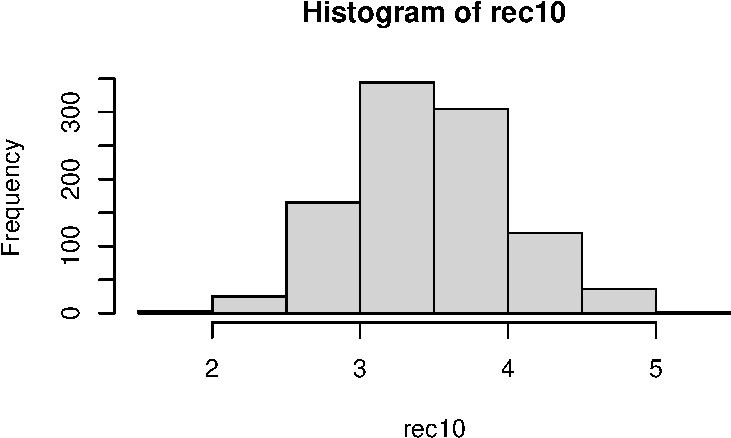
\includegraphics{6_hyohon_files/figure-pdf/unnamed-chunk-4-1.pdf}

}

\end{figure}

(毎回結果は変わりますが)この時最小値は1.8,最大値は5.3,平均は3.482でした。

これをサイコロを10000回振るのを1000回繰り返すのに変えてみます。

\begin{Shaded}
\begin{Highlighting}[]
\CommentTok{\#サイコロを10000回振るのを1000回繰り返す}
\NormalTok{S }\OtherTok{\textless{}{-}} \DecValTok{1000}
\NormalTok{rec10000 }\OtherTok{\textless{}{-}} \FunctionTok{numeric}\NormalTok{(S)}
\ControlFlowTok{for}\NormalTok{(i }\ControlFlowTok{in} \DecValTok{1}\SpecialCharTok{:}\NormalTok{S)\{}
\NormalTok{  rec10000[i] }\OtherTok{\textless{}{-}} \FunctionTok{sample}\NormalTok{(}\DecValTok{1}\SpecialCharTok{:}\DecValTok{6}\NormalTok{, }\DecValTok{10000}\NormalTok{, }\AttributeTok{replace =} \ConstantTok{TRUE}\NormalTok{)}\SpecialCharTok{|\textgreater{}}
    \FunctionTok{mean}\NormalTok{()}
\NormalTok{\}}
\FunctionTok{summary}\NormalTok{(rec10000)}
\end{Highlighting}
\end{Shaded}

\begin{verbatim}
   Min. 1st Qu.  Median    Mean 3rd Qu.    Max. 
  3.438   3.489   3.500   3.501   3.512   3.566 
\end{verbatim}

すると,最小値3.450,最大値3.553,平均値3.449と,3.5にかなり収束しました。

\begin{Shaded}
\begin{Highlighting}[]
\CommentTok{\#サイコロを100回振るのを1000回繰り返す}
\NormalTok{S }\OtherTok{\textless{}{-}} \DecValTok{1000}
\NormalTok{rec100 }\OtherTok{\textless{}{-}} \FunctionTok{numeric}\NormalTok{(S)}
\ControlFlowTok{for}\NormalTok{(i }\ControlFlowTok{in} \DecValTok{1}\SpecialCharTok{:}\NormalTok{S)\{}
\NormalTok{  rec100[i] }\OtherTok{\textless{}{-}} \FunctionTok{sample}\NormalTok{(}\DecValTok{1}\SpecialCharTok{:}\DecValTok{6}\NormalTok{, }\DecValTok{100}\NormalTok{, }\AttributeTok{replace =} \ConstantTok{TRUE}\NormalTok{)}\SpecialCharTok{|\textgreater{}}
    \FunctionTok{mean}\NormalTok{()}
\NormalTok{\}}

\CommentTok{\#3つそれぞれヒストグラムを書いて,}
\CommentTok{\#一つのシートに重ねて表示}
\FunctionTok{hist}\NormalTok{(rec10000, }
     \AttributeTok{col=}\StringTok{"\#FF00007F"}\NormalTok{, }
     \AttributeTok{xlim=}\FunctionTok{c}\NormalTok{(}\FloatTok{1.5}\NormalTok{,}\DecValTok{5}\NormalTok{),}
     \AttributeTok{ann=}\NormalTok{F, }
     \AttributeTok{main=}\StringTok{""}\NormalTok{, }
     \AttributeTok{xlab=}\StringTok{""}\NormalTok{ ,}
     \AttributeTok{breaks=}\FunctionTok{seq}\NormalTok{(}\DecValTok{1}\NormalTok{,}\DecValTok{6}\NormalTok{,}\FloatTok{0.1}\NormalTok{)}
\NormalTok{     )}
\FunctionTok{par}\NormalTok{(}\AttributeTok{new=}\NormalTok{T)}
\FunctionTok{hist}\NormalTok{(rec10, }
     \AttributeTok{breaks=}\FunctionTok{seq}\NormalTok{(}\DecValTok{1}\NormalTok{,}\DecValTok{6}\NormalTok{,}\FloatTok{0.1}\NormalTok{),}
     \AttributeTok{col=}\StringTok{"\#0000FF7F"}\NormalTok{,}
     \AttributeTok{ann=}\NormalTok{F, }
     \AttributeTok{add=}\NormalTok{T)}
\FunctionTok{hist}\NormalTok{(rec100, }
     \AttributeTok{breaks=}\FunctionTok{seq}\NormalTok{(}\DecValTok{1}\NormalTok{,}\DecValTok{6}\NormalTok{,}\FloatTok{0.1}\NormalTok{),}
     \AttributeTok{col=}\StringTok{"\#32CD32"}\NormalTok{,}
     \AttributeTok{ann=}\NormalTok{F, }
     \AttributeTok{add=}\NormalTok{T)}
\FunctionTok{legend}\NormalTok{(}\StringTok{"topright"}\NormalTok{, }
       \AttributeTok{legend=}\FunctionTok{c}\NormalTok{(}\StringTok{"rec10000"}\NormalTok{, }
                \StringTok{"rec10"}\NormalTok{, }
                \StringTok{"rec100"}\NormalTok{),}
       \AttributeTok{fill=}\FunctionTok{c}\NormalTok{(}\StringTok{"\#FF00007F"}\NormalTok{, }
              \StringTok{"\#0000FF7F"}\NormalTok{,}
              \StringTok{"\#32CD32"}\NormalTok{)}
\NormalTok{       )}
\end{Highlighting}
\end{Shaded}

\begin{figure}[H]

{\centering 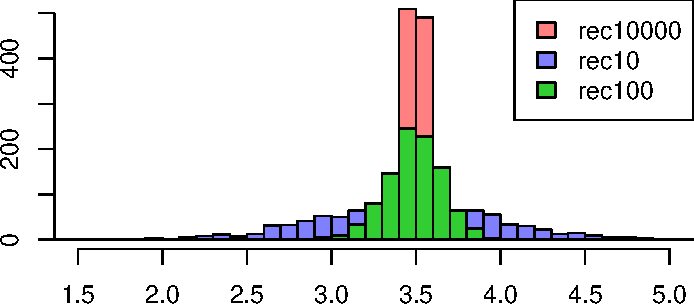
\includegraphics{6_hyohon_files/figure-pdf/unnamed-chunk-6-1.pdf}

}

\end{figure}

サンプルサイズ100のものも加えてヒストグラムを書きました。一回一回のサンプルサイズが大きいほど,母平均に近い値を取っていることが見えます。

\hypertarget{ux6a19ux672cux5206ux6563ux306eux6027ux8cea}{%
\section{標本分散の性質}\label{ux6a19ux672cux5206ux6563ux306eux6027ux8cea}}

標本分散や標準偏差についても大数の法則が成立します

\hypertarget{ux30b7ux30dfux30e5ux30ecux30fcux30b7ux30e7ux30f3}{%
\subsection{シミュレーション}\label{ux30b7ux30dfux30e5ux30ecux30fcux30b7ux30e7ux30f3}}

\begin{Shaded}
\begin{Highlighting}[]
\NormalTok{S }\OtherTok{\textless{}{-}} \DecValTok{1000}

\NormalTok{srec10 }\OtherTok{\textless{}{-}} \FunctionTok{numeric}\NormalTok{(S)}
\ControlFlowTok{for}\NormalTok{(i }\ControlFlowTok{in} \DecValTok{1}\SpecialCharTok{:}\NormalTok{S)\{}
\NormalTok{  srec10[i] }\OtherTok{\textless{}{-}} \FunctionTok{sd}\NormalTok{(}\FunctionTok{rnorm}\NormalTok{(}\DecValTok{10}\NormalTok{,}\DecValTok{50}\NormalTok{,}\DecValTok{10}\NormalTok{))}
\NormalTok{\}}

\NormalTok{srec100 }\OtherTok{\textless{}{-}} \FunctionTok{numeric}\NormalTok{(S)}
\ControlFlowTok{for}\NormalTok{(i }\ControlFlowTok{in} \DecValTok{1}\SpecialCharTok{:}\NormalTok{S)\{}
\NormalTok{  srec100[i] }\OtherTok{\textless{}{-}} \FunctionTok{sd}\NormalTok{(}\FunctionTok{rnorm}\NormalTok{(}\DecValTok{100}\NormalTok{,}\DecValTok{50}\NormalTok{,}\DecValTok{10}\NormalTok{))}
\NormalTok{\}}


\NormalTok{srec10000 }\OtherTok{\textless{}{-}} \FunctionTok{numeric}\NormalTok{(S)}
\ControlFlowTok{for}\NormalTok{(i }\ControlFlowTok{in} \DecValTok{1}\SpecialCharTok{:}\NormalTok{S)\{}
\NormalTok{  srec10000[i] }\OtherTok{\textless{}{-}} \FunctionTok{sd}\NormalTok{(}\FunctionTok{rnorm}\NormalTok{(}\DecValTok{10000}\NormalTok{,}\DecValTok{50}\NormalTok{,}\DecValTok{10}\NormalTok{))}
\NormalTok{\}}



\FunctionTok{hist}\NormalTok{(srec10000, }\AttributeTok{col=}\StringTok{"\#FF00007F"}\NormalTok{, }\AttributeTok{xlim=}\FunctionTok{c}\NormalTok{(}\DecValTok{1}\NormalTok{,}\DecValTok{18}\NormalTok{),}\AttributeTok{ann=}\NormalTok{F, }\AttributeTok{main=}\StringTok{""}\NormalTok{, }\AttributeTok{xlab=}\StringTok{""}\NormalTok{ ,}\AttributeTok{breaks=}\FunctionTok{seq}\NormalTok{(}\DecValTok{1}\NormalTok{,}\DecValTok{20}\NormalTok{,}\DecValTok{1}\NormalTok{))}
\FunctionTok{par}\NormalTok{(}\AttributeTok{new=}\NormalTok{T)}
\FunctionTok{hist}\NormalTok{(srec10, }\AttributeTok{breaks=}\FunctionTok{seq}\NormalTok{(}\DecValTok{1}\NormalTok{,}\DecValTok{20}\NormalTok{,}\DecValTok{1}\NormalTok{),}\AttributeTok{col=}\StringTok{"\#0000FF7F"}\NormalTok{,}\AttributeTok{ann=}\NormalTok{F, }\AttributeTok{add=}\NormalTok{T)}

\FunctionTok{hist}\NormalTok{(srec100, }\AttributeTok{breaks=}\FunctionTok{seq}\NormalTok{(}\DecValTok{1}\NormalTok{,}\DecValTok{20}\NormalTok{,}\DecValTok{1}\NormalTok{),}\AttributeTok{col=}\StringTok{"\#32CD32"}\NormalTok{,}\AttributeTok{ann=}\NormalTok{F, }\AttributeTok{add=}\NormalTok{T)}
\FunctionTok{legend}\NormalTok{(}\StringTok{"topright"}\NormalTok{, }\AttributeTok{legend=}\FunctionTok{c}\NormalTok{(}\StringTok{"rec10000"}\NormalTok{, }\StringTok{"rec10"}\NormalTok{, }\StringTok{"rec100"}\NormalTok{),}\AttributeTok{fill=}\FunctionTok{c}\NormalTok{(}\StringTok{"\#FF00007F"}\NormalTok{, }\StringTok{"\#0000FF7F"}\NormalTok{,}\StringTok{"\#32CD32"}\NormalTok{))}
\end{Highlighting}
\end{Shaded}

\begin{figure}[H]

{\centering 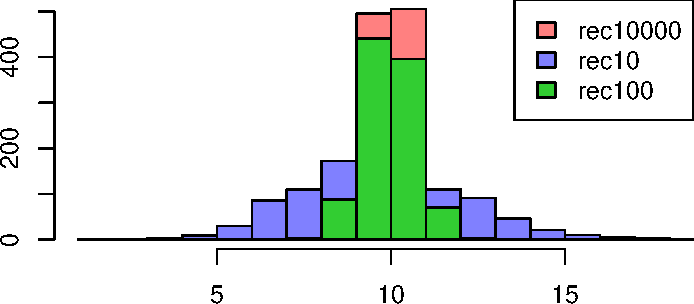
\includegraphics{6_hyohon_files/figure-pdf/unnamed-chunk-7-1.pdf}

}

\end{figure}



\end{document}
